% ASSIGNMENT 1 RANDOM SIGNALS AND STOCHASTIC PROCESSES

\setcounter{page}{1}

\section{Random Signals and Stochastic Processes}

\lhead{Advanced Signal Processing}
\rhead{Random Signals and Stochastic Processes}

% 1.1 Statistical Estimation
\subsection{Statistical Estimation}

A 1000-sample vector $\textbf{x}$ where each sample was a realisation of a uniform random variable $X \sim \textit{U}[0,1]$ was created and plotted, obtaining the plot in Figure \ref{fig:uniform1}.

\begin{figure}[H]
    \centering
    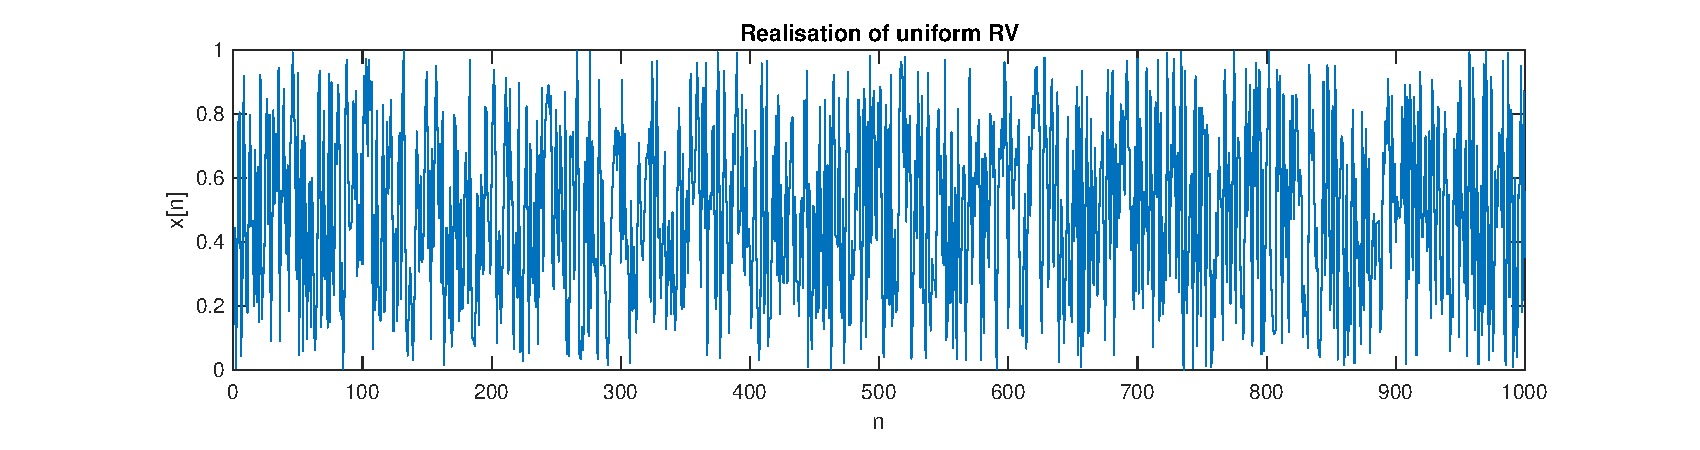
\includegraphics[width=14cm]{assignment1figs/uni_1.eps}
    \caption{1000-sample realisation of uniformly distributed random process $\textbf{x}$}
    \label{fig:uniform1}
\end{figure}

\subsubsection{Mean}

The theoretical mean $m$ can be calculated using using Equation \ref{eqn:mean1}.

\begin{equation}
    m = \int_{\infty}^{\infty}xp(x)dx
    \label{eqn:mean1}
\end{equation}

\noindent
Since $p(x)$ $\sim \textit{U}[0,1]$ is a uniform normal distribution, $x$ has a constant value of 1 in limits [0,1] and 0 elsewhere. With this insight, the following result is obtained:

\begin{equation}
    m = \int_{0}^{1}xdx = 0.5
    \label{eqn:mean2}
\end{equation}

\noindent
Using MATLAB's \code{mean()} function, the sample mean $\hat{m}$ was calculated with slight variation each time. Table \ref{tab:uni_mean} shows the results obtained for 5 instances of this random process.
 
\begin{table}[H]
\centering
\begin{tabular}{C{3cm} C{2cm}}
\Xhline{2\arrayrulewidth}
\textbf{Sample mean} & \textbf{Error} \\ \Xhline{2\arrayrulewidth}
0.5045 & -0.0045 \\ 
0.4971 & 0.0029 \\ 
0.5038 & -0.0038 \\ 
0.4977 & 0.0023 \\ 
0.4928 & 0.0058 \\ 
\hline
\end{tabular}
\caption{Sample means and error.}
\label{tab:uni_mean}
\end{table}

\noindent
It is clear that the sample mean $\hat{m}$ is an accurate estimator for the theoretical/true mean $m$ up to 2 decimal places.

\subsubsection{Standard Deviation}

A similar process can used to compare the theoretical and sample SD. The theoretical SD $\sigma$ can be calculated using Equation (3).

\begin{center}
\begin{equation}
    \sigma = \sqrt{E(X^2)-(E(X))^2}
    \end{equation} \begin{equation}
    = \sqrt{\int_0^1x^2dx - (\frac{1}{2})^2}
    \end{equation} \begin{equation}
    = \sqrt{\frac{1}{3} - \frac{1}{4}}
    \end{equation} \begin{equation}
    = \sqrt{\frac{1}{12}}
    \end{equation} \begin{equation}
    = 0.2887
\end{equation}
\end{center}

\noindent
Using MATLAB's \code{std()} function, the sample SD $\hat{\sigma}$ was calculated with slight variation each time. Table \ref{tab:uni_sd} shows the results obtained for 5 instances of this random process.

\begin{table}[H]
\centering
\begin{tabular}{C{3cm} C{2cm}}
\Xhline{2\arrayrulewidth}
\textbf{Sample SD} & \textbf{Error} \\ \Xhline{2\arrayrulewidth}
0.2834 & 0.0053 \\ 
0.2845 & 0.0041 \\ 
0.2908 & -0.0021 \\ 
0.2840 & 0.0046 \\ 
0.2909 & -0.0023 \\ 
\hline
\end{tabular}
\caption{Sample SDs and error.}
\label{tab:uni_sd}
\end{table}

\noindent
Like the mean, it is clear that the sample SD $\hat{\sigma}$ is an accurate estimator for the theoretical/true SD $\sigma$ up to 2 decimal places. As the number of samples is increased, the sample statistics will converge to the theoretical statistics. 

\subsubsection{Bias}

An ensemble of 10 realisations of $\textbf{x}$ was generated and then the procedure outlined above was repeated to calculate the sample means and SDs for each realisation. Plots illustrating the theoretical values in red are shown in Figure \ref{fig:samplevals1}.

\begin{figure}[H]
    \centering
    \subfloat[Sample means]{{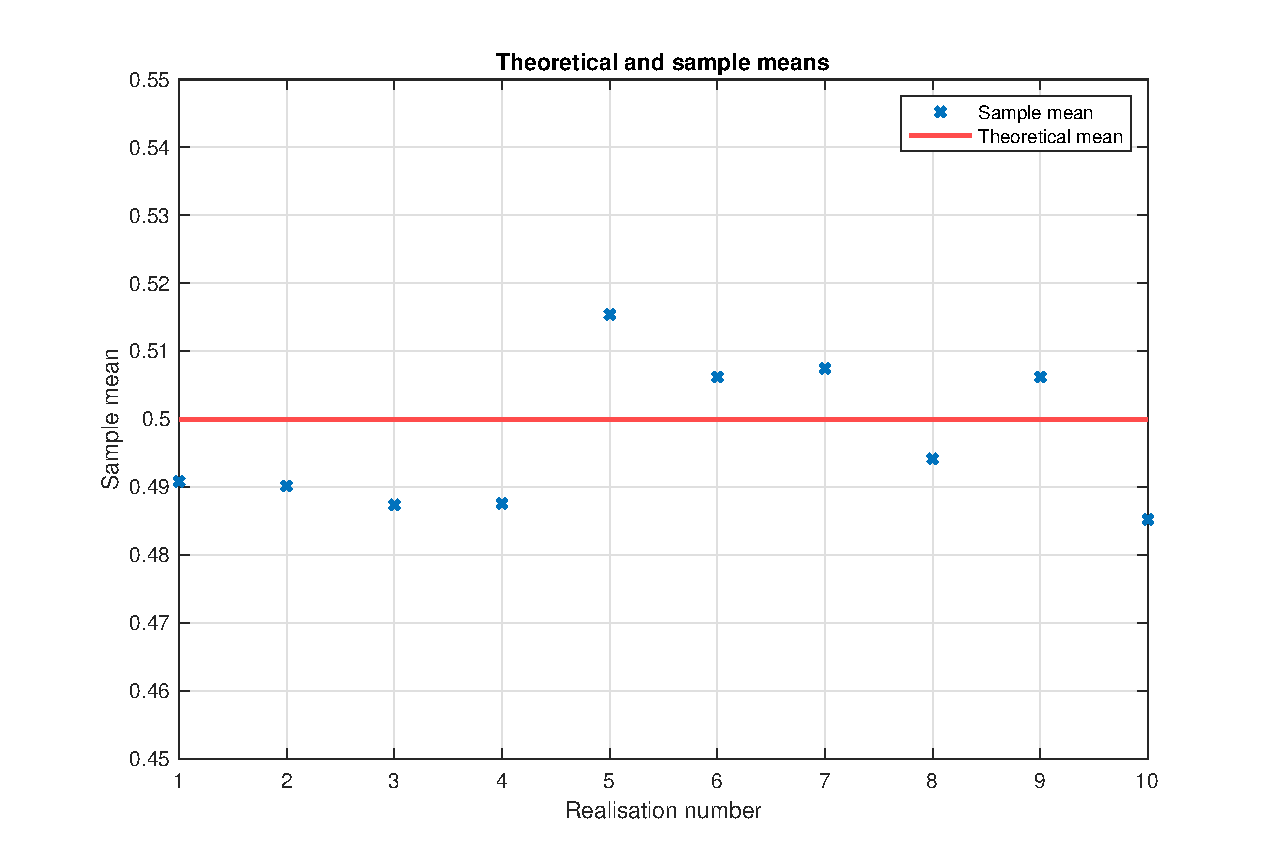
\includegraphics[width=6.5cm]{assignment1figs/uni_mean.eps}}}
    \subfloat[Sample SDs]{{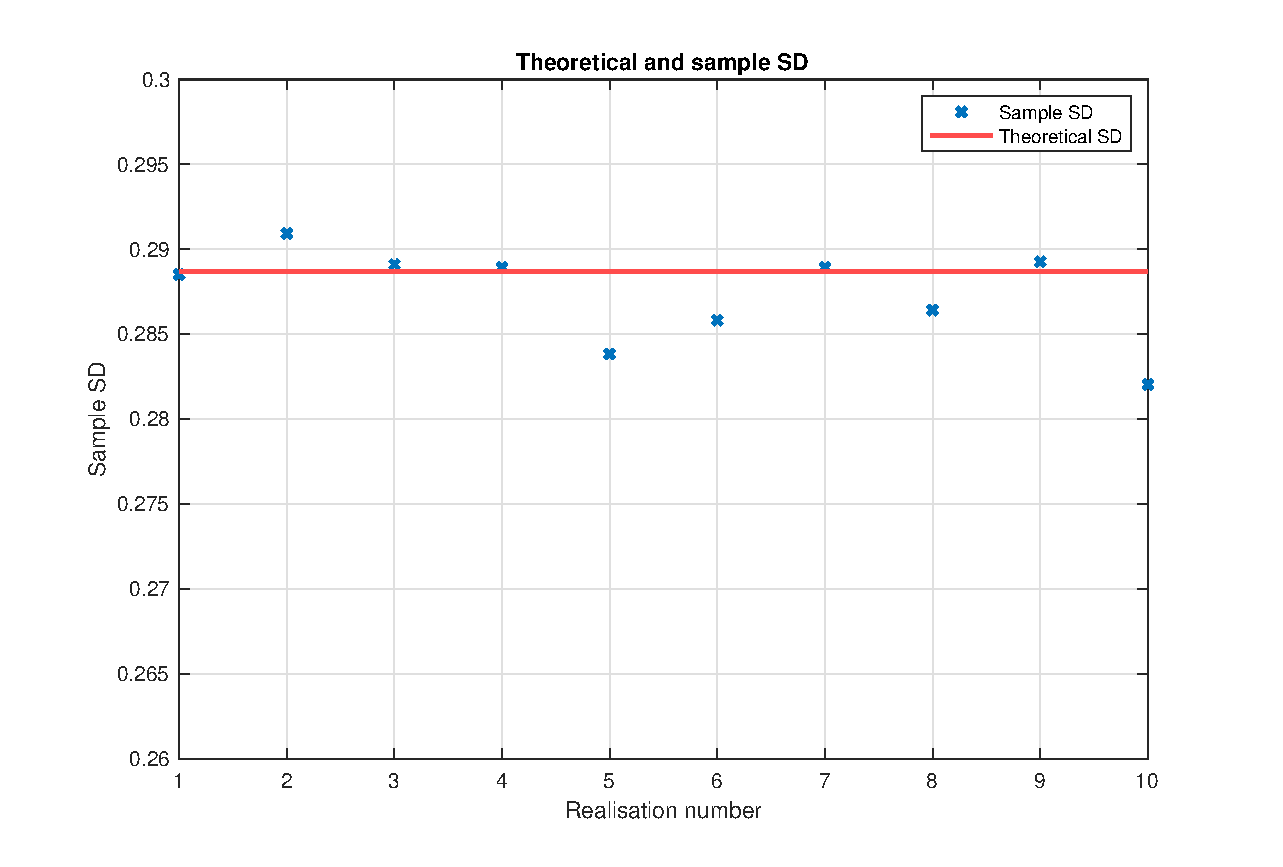
\includegraphics[width=6.5cm]{assignment1figs/uni_SD.eps}}}
    \caption{Sample statistics for $\textbf{x}_{1:10}$ with uniform RV}
    \label{fig:samplevals1}
\end{figure}

\noindent
The sample statistics clearly have a tendency to cluster around the theoretical statistics, implying that the sample mean $\hat{m}$ and SD $\hat{\sigma}$ are both unbiased estimators for the theoretical statistics. However, the sample size of 10 is too small to make any meaningful inferences, and this would need to be repeated with more samples to be sure.

\subsubsection{PDF Estimation}
The histogram of a realisation of $x$ acts as an approximation of the theoretical pdf since the y-axis represents frequency and therefore when normalised by total number of counts is analogous to probability.

\begin{figure}[H]
    \centering
    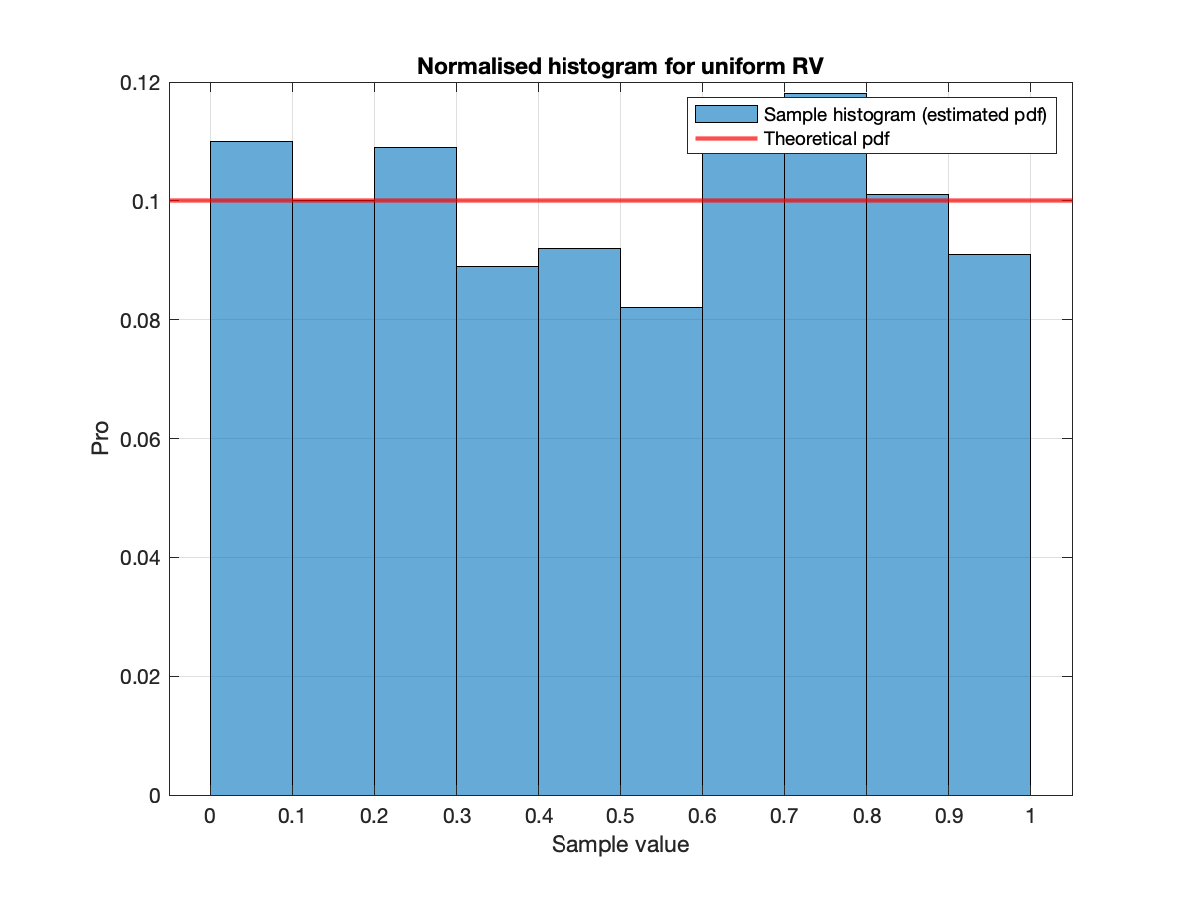
\includegraphics[width=6.5cm]{assignment1figs/unihist.eps}
    \caption{1000-sample realisation of uniformly distributed random process $X \sim \textit{U}[0,1]$}
    \label{fig:unihist}
\end{figure}

\noindent
As the number of samples is increased, the accuracy of the approximation improves, and the histogram tends towards the uniform distribution, which has been overlaid in red. Since the total theoretical probability is 1 and there are 10 bins, the value of each bin must tend to 0.1, such that the area under the distribution is 1. If the number of bins is increased, the value that each tends towards changes according to the relationship given by Equation \ref{eqn:bins}.

\begin{equation}
    P_{bin} = \frac{1}{n_{bins}}
    \label{eqn:bins}
\end{equation}

\subsubsection{Using a Gaussian random variable}
This analysis was repeated drawing the 1000 samples of the random variable from a Gaussian distribution, i.e.  $X \sim \textit{N}[0,1]$. 
\\\\
By definition, the theoretical mean $m$ of the standard normal distribution is 0. It was found that the sample mean $\hat{m}$ is an accurate estimator of the theoretical mean $m$ to 1 decimal place.
\\\\
By definition, the theoretical SD $\sigma$ of a standard normal distribution is 1. It was found that the sample SD $\hat{\sigma}$ is, on average, an accurate estimator of the theoretical SD $\sigma$ to 1 decimal place.
\\\\
The bias of the estimated values for mean and SD can be estimated using the same approach as before, as demonstrated by Figure \ref{fig:samplevals2}.
\\\\
\begin{figure}[H]
    \centering
    \subfloat[Sample means]{{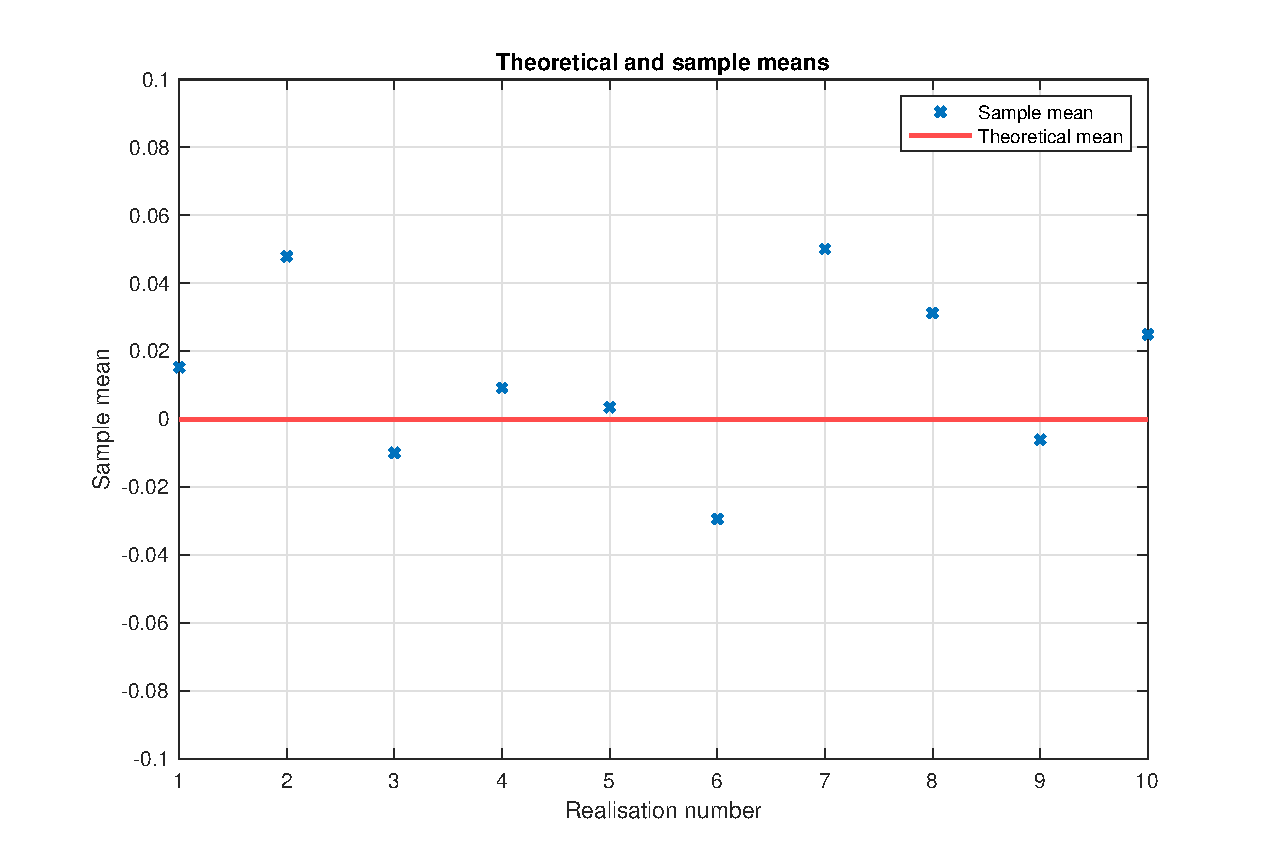
\includegraphics[width=6.5cm]{assignment1figs/gauss_mean.eps}}}
    \subfloat[Sample SDs]{{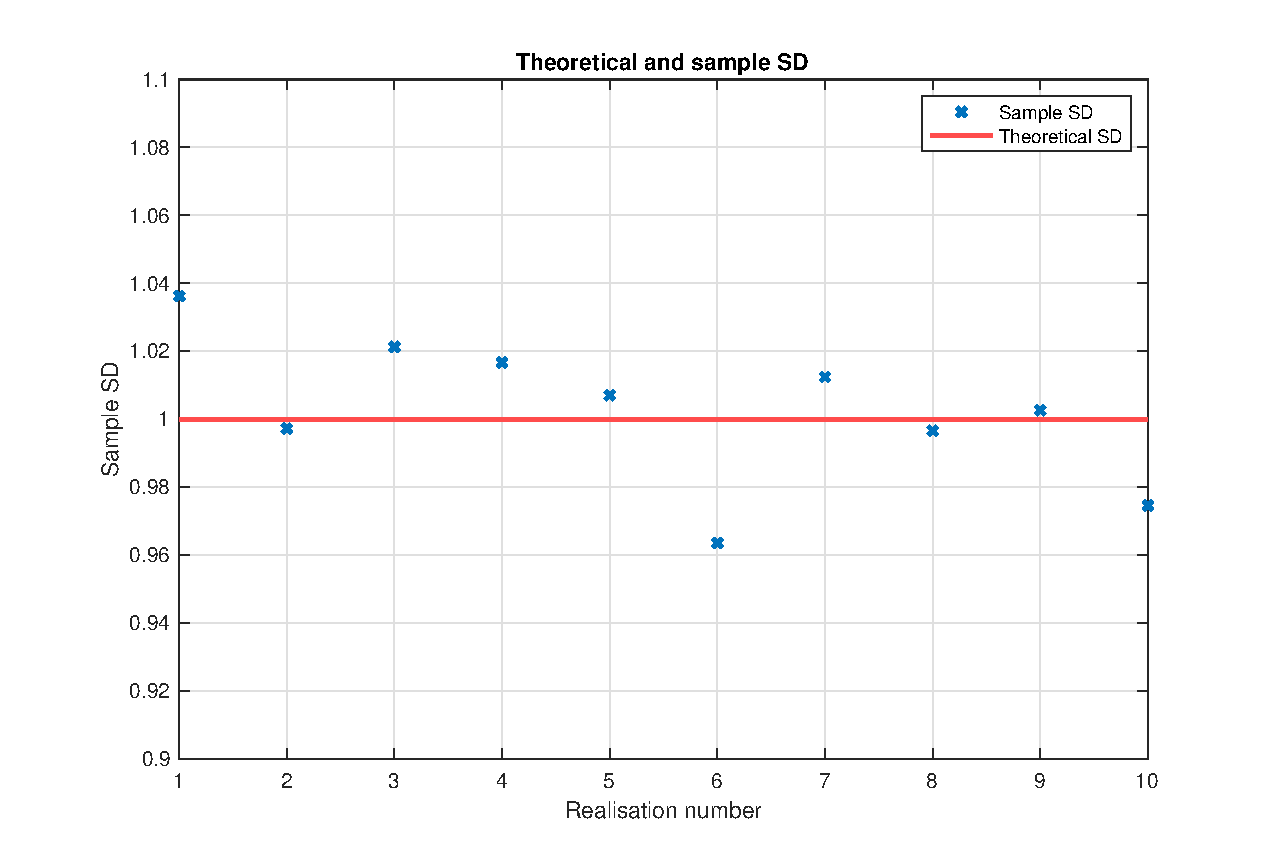
\includegraphics[width=6.5cm]{assignment1figs/gauss_sd.eps}}}
    \caption{Sample statistics for $\textbf{x}_{1:10}$ with Gaussian RV}
    \label{fig:samplevals2}
\end{figure}

\noindent
There is no clear bias in the estimate for mean or SD in this case. However, it is noteworthy that the sample mean $\hat{m}$ appears to be a less accurate estimator for this Gaussian normal distribution than for the uniform distribution, with a maximum error of $\approx$0.01 for the uniformly distributed process but $\approx$0.05 for this Gaussian process.
\\\\\noindent
An estimate of the PDF can be obtained from the normalised histogram in the same manner as before and is displayed in Figure \ref{fig:gausshist}. (This time, the \code{bar()} function was used rather than the \code{histogram()} function, hence the slightly different appearance).

\begin{figure}[H]
    \centering
    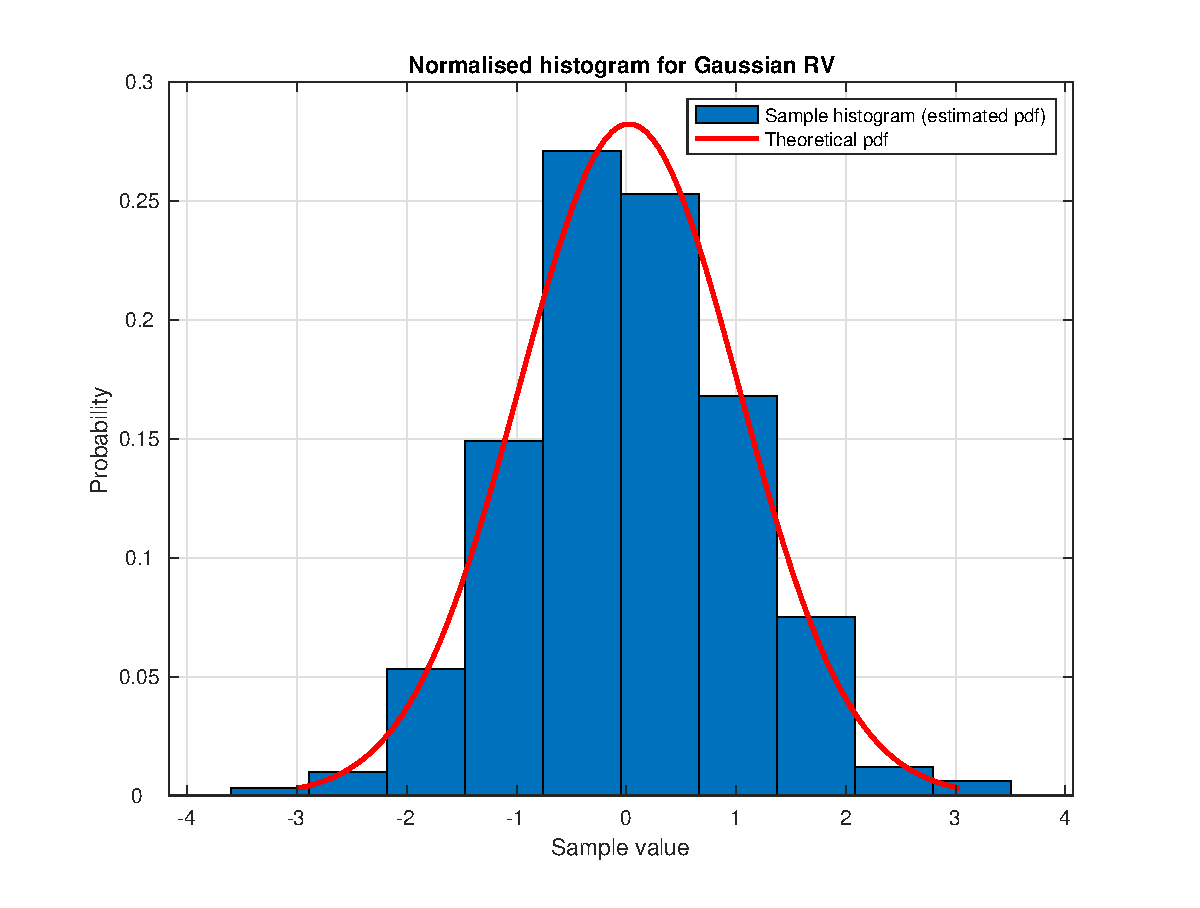
\includegraphics[width=7.5cm]{assignment1figs/gausshist.eps}
    \caption{1000-sample realisation of Gaussian distributed random process $x \sim \textit{N}[0,1]$}
    \label{fig:gausshist}
\end{figure}

\noindent
As before, as the number of samples is increased, the accuracy of the approximation improves, and the histogram tends towards the Gaussian standard normal distribution, which has been overlaid in red.

% 1.2 Stochastic Processes
\subsection{Stochastic processes}

Stochasticity, stationarity and ergodicity are three of the most important concepts in statistical signal processing, and are therefore defined below for clarity.

\begin{itemize}
\item A \textit{stochastic} process is as a collection of random variables.
\item A \textit{stationary} process is a random process whose statistical properties are constant in time.
\item An \textit{ergodic} process is one in which the time average is equal to the ensemble average. The same result is obtained for statistical properties of one process realisation in time as from all realisations at a single time instant.
\end{itemize}

\noindent
We were given 3 random processes to analysed, which I will refer to as 'RP1', 'RP2, and 'RP3'. Ensembles of 100 realisations of these random processes, each of length 100 samples were generated. 

\subsubsection{Stationarity}

To analyse stationarity, ensemble means and SDs of each process were plotted against time, as shown in Figure \ref{fig:rps}. 

\begin{figure}[H]
    \begin{center}
\begin{subfigure}{0.4\textwidth}
  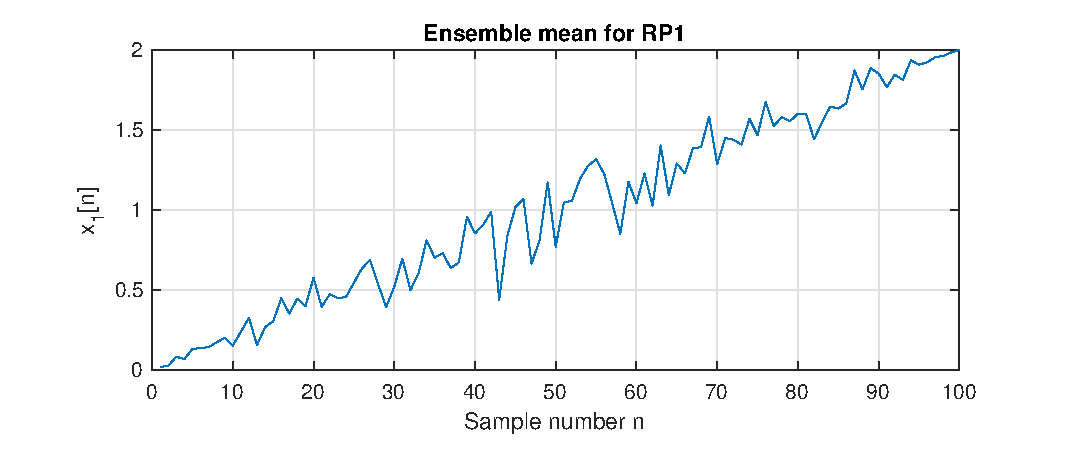
\includegraphics[width=\linewidth]{assignment1figs/RP1_mean.eps}
  \caption{RP1 mean.}
  \label{fig:rp1mean}
\end{subfigure}\hfil 
\begin{subfigure}{0.4\textwidth}
  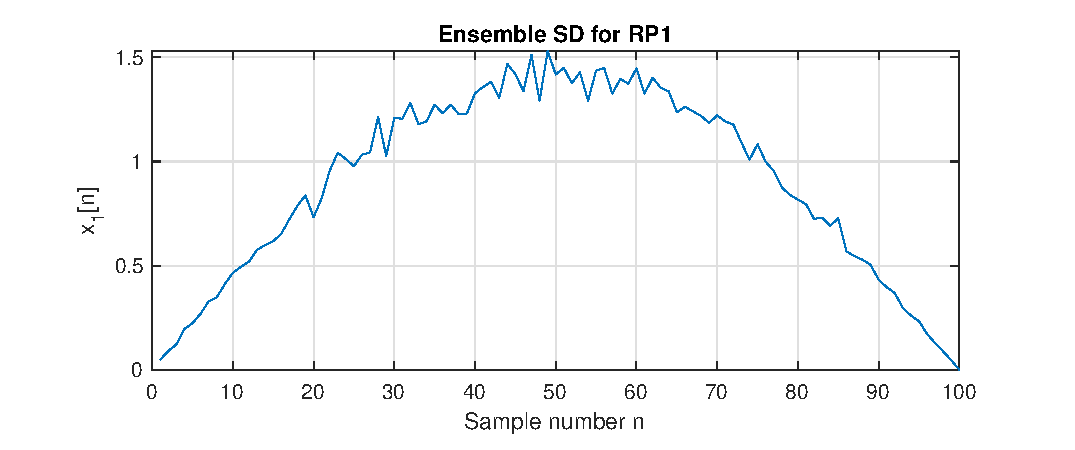
\includegraphics[width=\linewidth]{assignment1figs/RP1_SD.eps}
  \caption{RP1 SD.}
  \label{fig:rp1SD}
\end{subfigure}
\medskip
\begin{subfigure}{0.4\textwidth}
  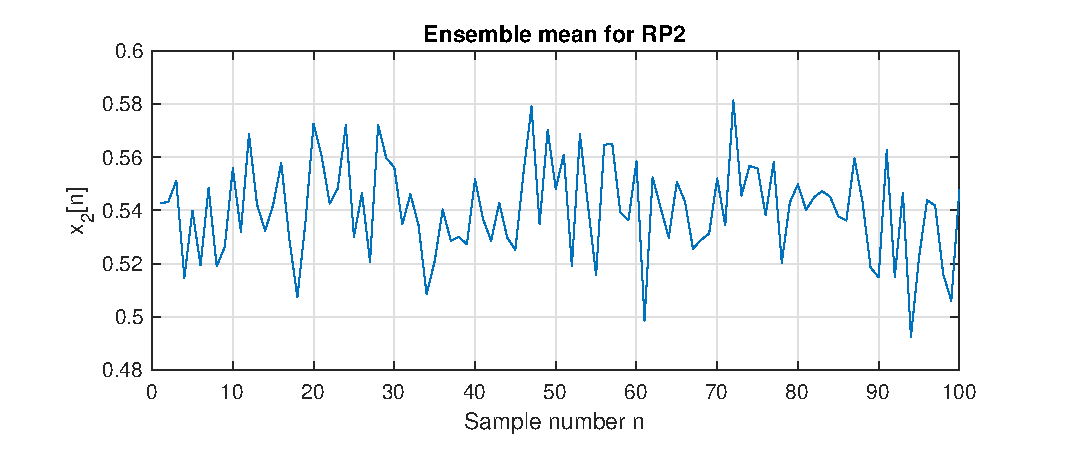
\includegraphics[width=\linewidth]{assignment1figs/RP2_mean.eps}
  \caption{RP2 mean.}
  \label{fig:rp2mean}
\end{subfigure}\hfil 
\begin{subfigure}{0.4\textwidth}
  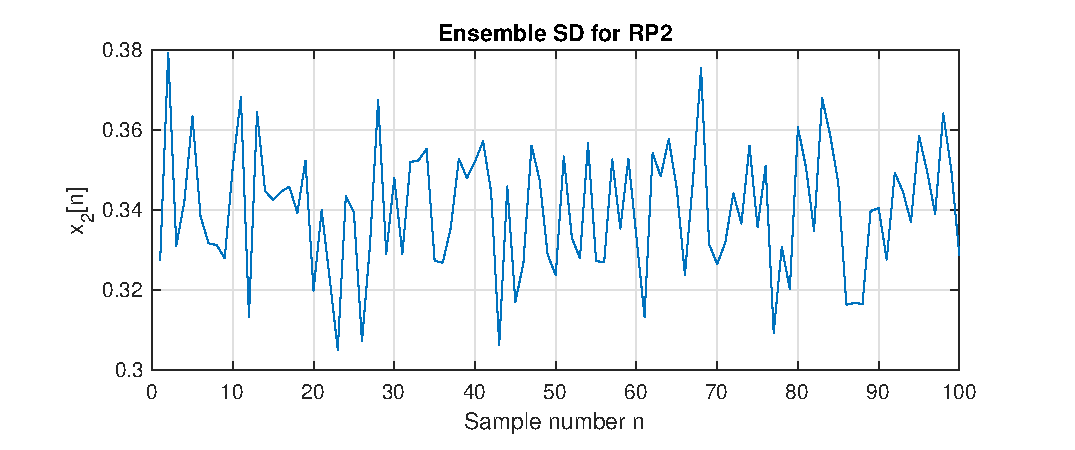
\includegraphics[width=\linewidth]{assignment1figs/RP2_SD.eps}
  \caption{RP2 SD.}
  \label{fig:rp2SD}
\end{subfigure}
\medskip
\begin{subfigure}{0.4\textwidth}
  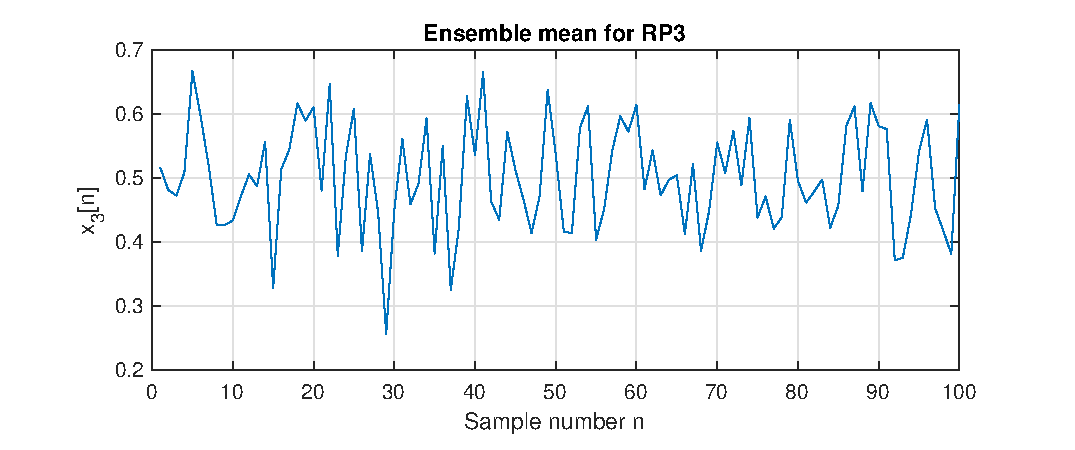
\includegraphics[width=\linewidth]{assignment1figs/RP3_mean.eps}
  \caption{RP3 mean.}
  \label{fig:rp3mean}
\end{subfigure}\hfil 
\begin{subfigure}{0.4\textwidth}
  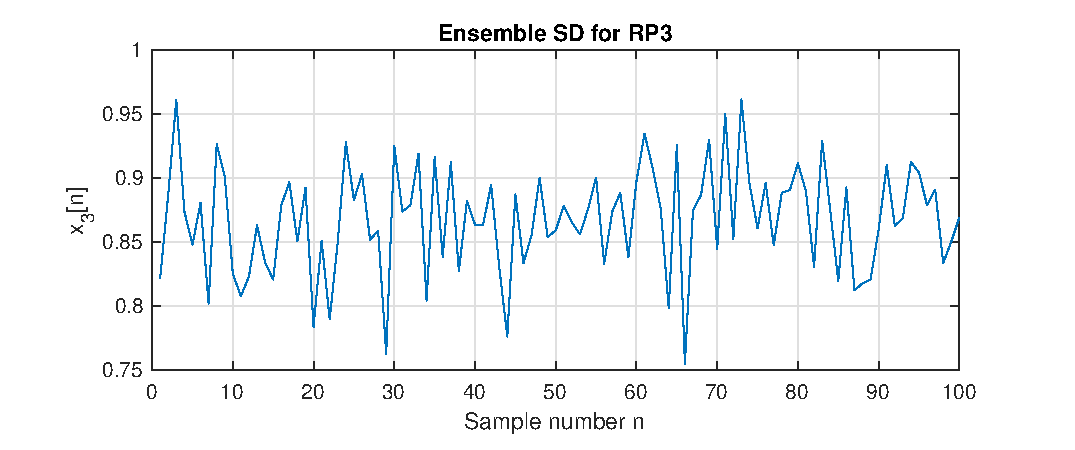
\includegraphics[width=\linewidth]{assignment1figs/RP3_SD.eps}
  \caption{RP3 SD.}
  \label{fig:rp3SD}
\end{subfigure}
\caption{Ensemble means and SDs for random processes}
\label{fig:rps}
\end{center}
\end{figure}

\noindent
It is immediately obvious that RP1 is non-stationary, since the ensemble mean $m_1[n]$ linearly increases from a value of 0 to a value of 2 and can be approximated by Equation \ref{eqn:meanrp1}.

\begin{equation}
    m_{1}[n] = \frac{n}{50}
    \label{eqn:meanrp1}
\end{equation}

\noindent
The ensemble SD $\sigma_{1}[n]$ also changes and can be approximated by Equation \ref{eqn:sdrp1}.

\begin{equation}
    \sigma_{1}[n] = 1.4sin(\frac{n\pi}{N})
    \label{eqn:sdrp1}
\end{equation}

\noindent
where N is the total number of samples (in this case N = 100).
\\\\
It is also clear that RP2 and RP3 are stationary, since there is no clear change in the mean and SD of either process. RP2 appears to have a mean $m_2$ of 0.54 and a SD $\sigma_2$ of 0.34. RP3 appears to have a mean $m_3$ of 0.50 and a SD $\sigma_3$ of 0.88.  

\subsubsection{Ergodicity for M=4, N=1000}

1000-sample realisations of the three random processes are created and the mean and SD are calculated for each realisation and displayed in Table \ref{Tab:ergod}.

\begin{table}[H]
\centering
\begin{tabular}{C{2.5cm} C{3cm}  C{3.5cm}  C{3.5cm}}
\Xhline{2\arrayrulewidth}
\textbf{Process}  & \textbf{Realisation} & \textbf{Mean} & \textbf{Standard Deviation} \\ \Xhline{2\arrayrulewidth}
\multirow{4}{*}{} & 1 & 9.2900 & 5.9025 \\ 
     \textbf{RP1} & 2 & 9.9936 & 5.8944 \\ 
                  & 3 & 9.9995 & 5.8690 \\  
                  & 4 & 10.0452 & 5.8515 \\ \hline
\multirow{4}{*}{} & 1 & 0.5756 & 0.0809 \\  
    \textbf{RP2}  & 2 & 0.4340 & 0.1515 \\  
                  & 3 & 0.9109 & 0.1420 \\  
                  & 4 & 0.5539 & 0.0444 \\ \hline
\multirow{4}{*}{} & 1 & 0.5324 & 0.8535 \\  
     \textbf{RP3} & 2 & 0.5171 & 0.8567 \\  
                  & 3 & 0.4860 & 0.8702 \\  
                  & 4 & 0.4757 & 0.8655 \\ \hline
\end{tabular}
\caption{Time means and SDs for different process realisations}
\label{Tab:ergod}
\end{table}

\noindent
The mean and SD of RP1 are roughly constant for each realisation. However, since this process is non-stationary, it cannot be ergodic since its statistical properties cannot be inferred from a single realisation.
\\\\
The mean and SD of RP2 vary considerably between realisations, implying that the statistical properties of the process cannot be inferred from a single realisation, regardless of the number of samples/ signal length and therefore implying that the process is not ergodic.
\\\\
The mean and SD of RP3 are roughly constant for each realisation and are also equal to the ensemble mean and SD values calculated in the previous part, implying that the process is ergodic.

\subsubsection{Mathematical Description for Process Means and SD}

Based on the MATLAB code provided, I was able to devise mathematical descriptions of each of the three stochastic processes.

\subsubsection*{RP1}

RP1 is defined by Equation \ref{eqn:rp1}

\begin{equation}
    x_{1}[n] = zb \times \sin \left(\frac{n \pi}{N}\right) + an
    \label{eqn:rp1}
\end{equation}

\noindent
where z $\sim$ U(-0.5,0.5), b = 5, a = 0.02 and N = total number of samples. Since $z \sim U(-0.5,0.5), E(z)$ = 0 and \textit{var}(z) =$ \frac{1}{\sqrt{12}}$.
\\\\
The theoretical mean can be calculated by applying the expectation operator, as below.

\begin{center}
\begin{equation}
    E(x_{1}[n]) = E(ub \sin \left(\frac{n \pi}{N}\right) + an) 
\end{equation}
\begin{equation}
= E(z)\times E(b \times \sin \left(\frac{n \pi}{N}\right)) + E(an) 
\end{equation}
\begin{equation}
= E(an) 
\end{equation}
\begin{equation}
= a \times E(n) 
\end{equation}
\begin{equation}
    = a \times n
\end{equation}
\begin{equation}
m_{1}= \frac{n}{50}
\end{equation}
\end{center}

\noindent
The theoretical SD can be calculated by applying the identity in Equation \ref{eqn:var}.

\begin{equation}
    \textit{var}(y) = E(y^2) - (E(y))^2
    \label{eqn:var}
\end{equation}
\begin{center}
\begin{equation}
    var(x_{1}[n]) = E({x_{1}[n]}^2) - (E({x_{1}[n]}))^2 
\end{equation}
\begin{equation}
= E(z^{2}b^{2}\sin^{2}(\frac{n \pi}{N}) + a^{2}n^{2}+2zb sin(\frac{n \pi}{N})an) - a^{2}n^{2}
\end{equation}
\begin{equation}
=E(z^{2} b^{2} \sin ^{2}(\frac{n \pi}{N}))+E(a^{2} n^{2})-a^{2} n^{2}
\end{equation}
\begin{equation}
=E(z^{2}) b^{2} \sin ^{2}(\frac{n \pi}{N})
\end{equation}
\begin{equation}
= \frac{1}{\sqrt{12}} b^{2} \sin ^{2}(\frac{n \pi}{N})
\end{equation}
\begin{equation}
\therefore \sigma_{1} =\sqrt{{var}(x_{1}[n])}
\end{equation}
\begin{equation}
=\frac{1}{\sqrt{12}} b \sin (\frac{n \pi}{N})
\end{equation}
\begin{equation}
\sigma_{1}=1.44 \times \sin \left(\frac{n \pi}{N}\right)
\end{equation}
\end{center}

\noindent
It is clear that both the calculated mean and SD agree with the observations in the previous section.

\subsubsection*{RP2}

RP2 is defined by Equation \ref{eqn:rp2}.

\begin{equation}
    x_{2}[n] = zM_{r} + A_{r}
    \label{eqn:rp2}
\end{equation}
where $M_{r}, A_{r} \sim U[0,1]$ and $z \sim U[-0.5,0.5]$. Immediately, we can say $E(M_{r}) = E(A_{r}) = 0.5$ and $E(z) = 0$, whilst the SD for all variables is $\frac{1}{\sqrt{12}}$.
\\\\
\noindent
Again, the theoretical mean can be calculated by applying the expectation operator, as below.

\begin{center}
\begin{equation}
E(x_{2}[n] )
\end{equation} \begin{equation}
= E(z)E(M_{r})+E(A_{r}) 
\end{equation} \begin{equation}
m_{2} = 0.5
\end{equation}
\end{center}

\noindent
The theoretical SD can again be calculated using the identity in Equation \ref{eqn:var}.

\begin{center}
\begin{equation}
var(x_{2}[n]) =  E({x_{2}[n]}^2) - (E({x_{2}[n]}))^2 
\end{equation} \begin{equation}
= E(A_{r}^{2}+2A_{r}M_{r}z+M_{r}^{2}z^{2}) - A_{r}^2
\end{equation} \begin{equation}
= E(A_{r}^{2})+ E(M_{r}^{2})E(z^{2}) - A_{r}^2
\end{equation} \begin{equation}
= \frac{1}{3} \times \frac{1}{36} - \frac{1}{4} = \frac{1}{9}
\end{equation} \begin{equation}
\therefore \sigma_{2} = \sqrt{\frac{1}{9}} = \frac{1}{3} = 0.333
\end{equation}
\end{center}

\noindent
Again, it is clear that both the calculated mean and SD agree with the observations in the previous section.

\subsubsection*{RP3}

RP3 is defined by Equation \ref{eqn:rp3}.

\begin{equation}
    x_{3}[n] = zm + a
    \label{eqn:rp3}
\end{equation}

\noindent
where m = 3, a = 0.5 and $z \sim U[-0.5,0.5]$. Therefore, clearly E(z) = 0.
\noindent
Again, the theoretical mean can be calculated by applying the expectation operator, as below.

\begin{center}
\begin{equation}
E(x_{3}[n]=mE(z)+a
\end{equation} \begin{equation}
m_{3} = 0.5
\end{equation}
\end{center}

\noindent
The theoretical SD can again be calculated using the identity in Equation \ref{eqn:var}.

\begin{center}
\begin{equation}
var(x_{3}[n])=E(x_{3}[n]^{2})-(E(x_{3}[n]))^{2}
\end{equation} \begin{equation}
=E(m^{2}z^{2}+a^{2}+2amz)-0.2
\end{equation} \begin{equation}
=0.75
\end{equation} \begin{equation}
\therefore \sigma_{3} = 0.867
\end{equation}
\end{center}
\noindent
Again, it is clear that both the calculated mean and SD agree with the observations in the previous section.

% 1.3 Estimation of Probability Distributions
\subsection{Estimation of probability distributions}

\subsubsection{PDF estimator function}

I wrote a MATLAB function to estimate the probability distribution function of a random process from its histogram. The code used in this function is shown below.
\\\\
\code{
\textcolor{blue}{function} pdf$\_$est(samples)\\
\textcolor{white}{....}histogram(samples,\textcolor{purple}{'BinWidth'},0.05,\textcolor{purple}{'Normalization'},\textcolor{purple}{'pdf'});grid \textcolor{purple}{on};\\
\textcolor{white}{....}xlabel(\textcolor{purple}{'Random Variable'});\\
\textcolor{white}{....}ylabel(\textcolor{purple}{'Probability'});\\
\textcolor{white}{....}title(\textcolor{purple}{'PDF Estimate for RV'});\\
\textcolor{blue}{end}}
\\\\
Testing the code on a 100-sample stationary Gaussian random process obtains the plot shown in Figure \ref{fig:pdfest1}. The PDF has been normalised such that its integral is 1.

\begin{figure}[H]
\begin{center}
    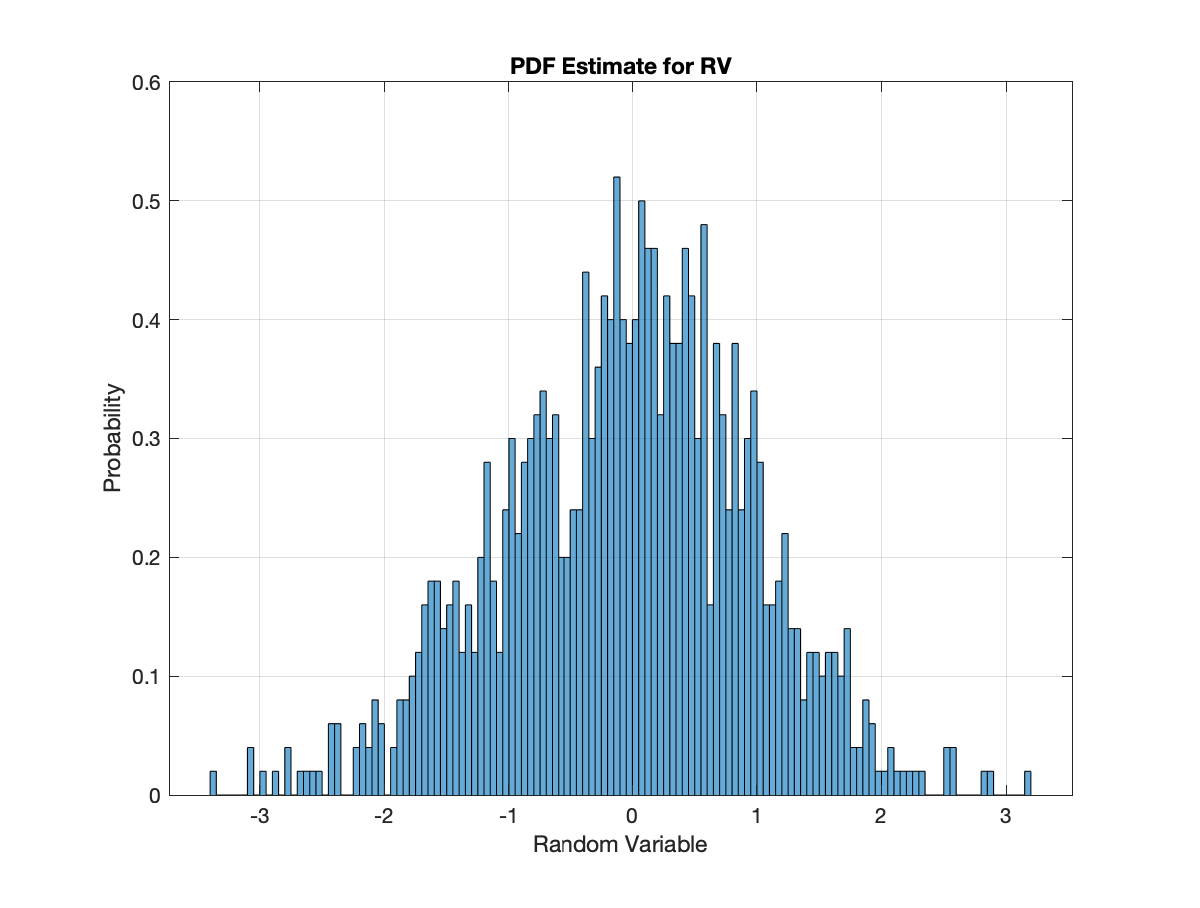
\includegraphics[width=8cm]{assignment1figs/gausspdf.eps}
    \caption{PDF estimator function applied to 1000-sample Gaussian process}
    \label{fig:pdfest1}
\end{center}
\end{figure}

\subsubsection{Effect of data length \textit{N}}

\noindent
The function was then tested on RP3 since it is both stationary and ergodic, obtaining the following plots for signal lengths of 100, 1000 and 10,000.
\begin{figure}[H]
\begin{subfigure}{.32\textwidth}
  \centering
  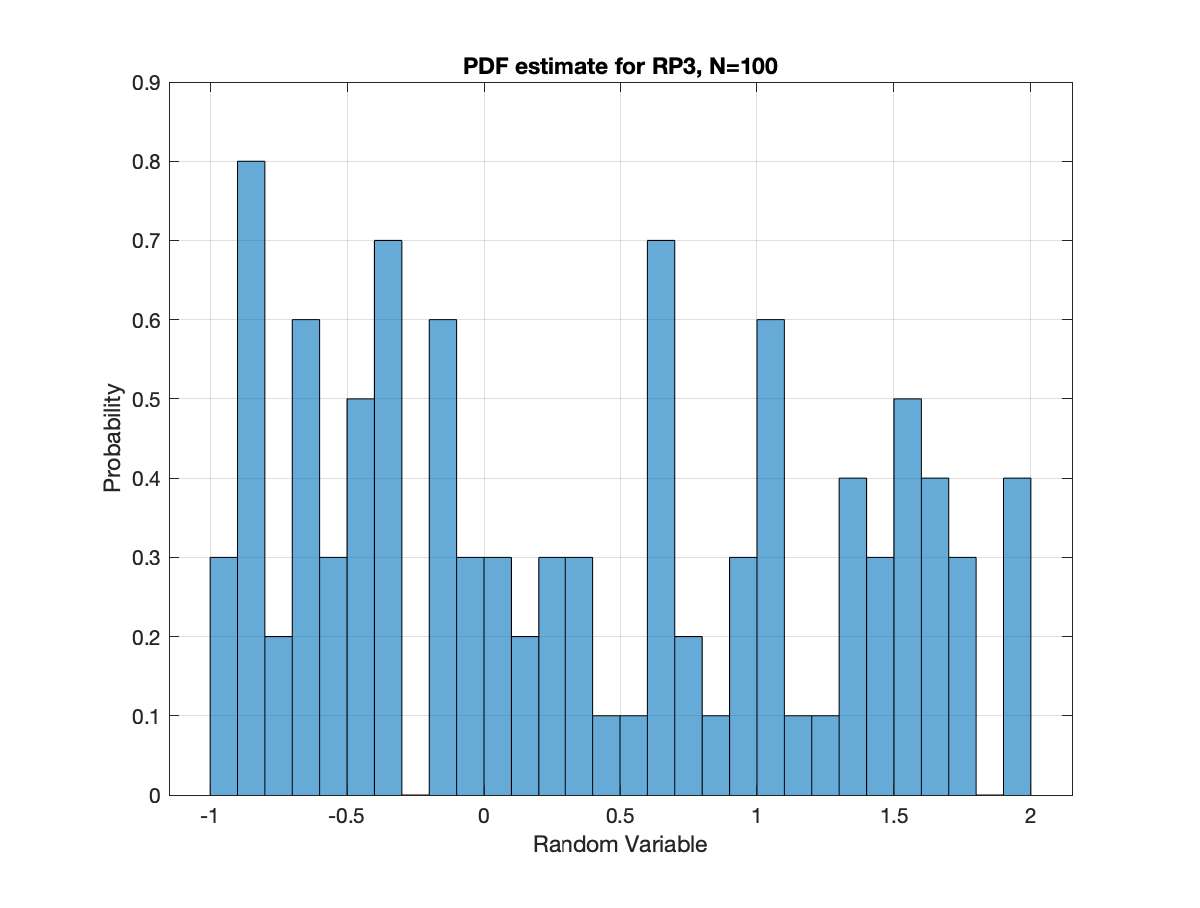
\includegraphics[width=\linewidth]{assignment1figs/rp3100}  
  \caption{100-sample realisation}
\end{subfigure}
\begin{subfigure}{.32\textwidth}
  \centering
  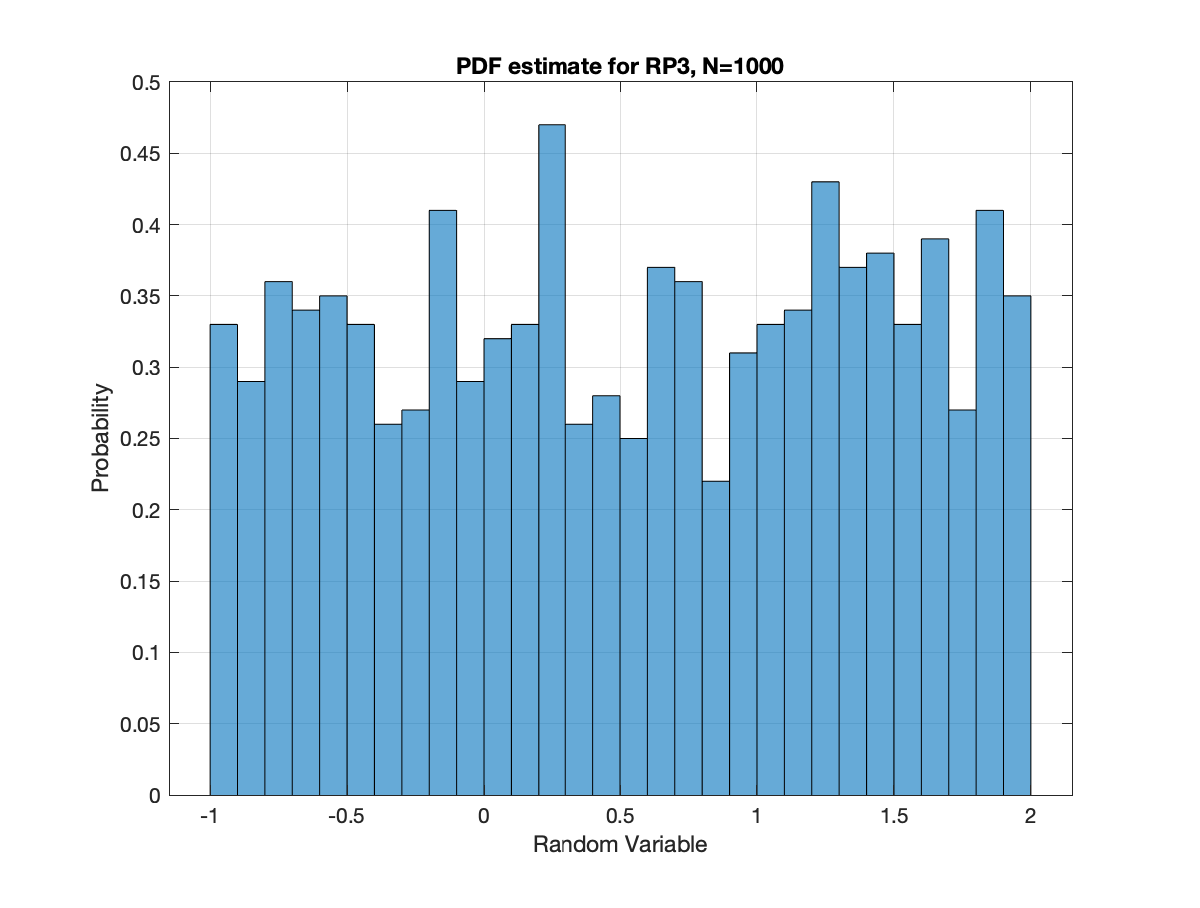
\includegraphics[width=\linewidth]{assignment1figs/rp31000.eps}  
  \caption{1000-sample realisation}
\end{subfigure}
\begin{subfigure}{.32\textwidth}
  \centering
  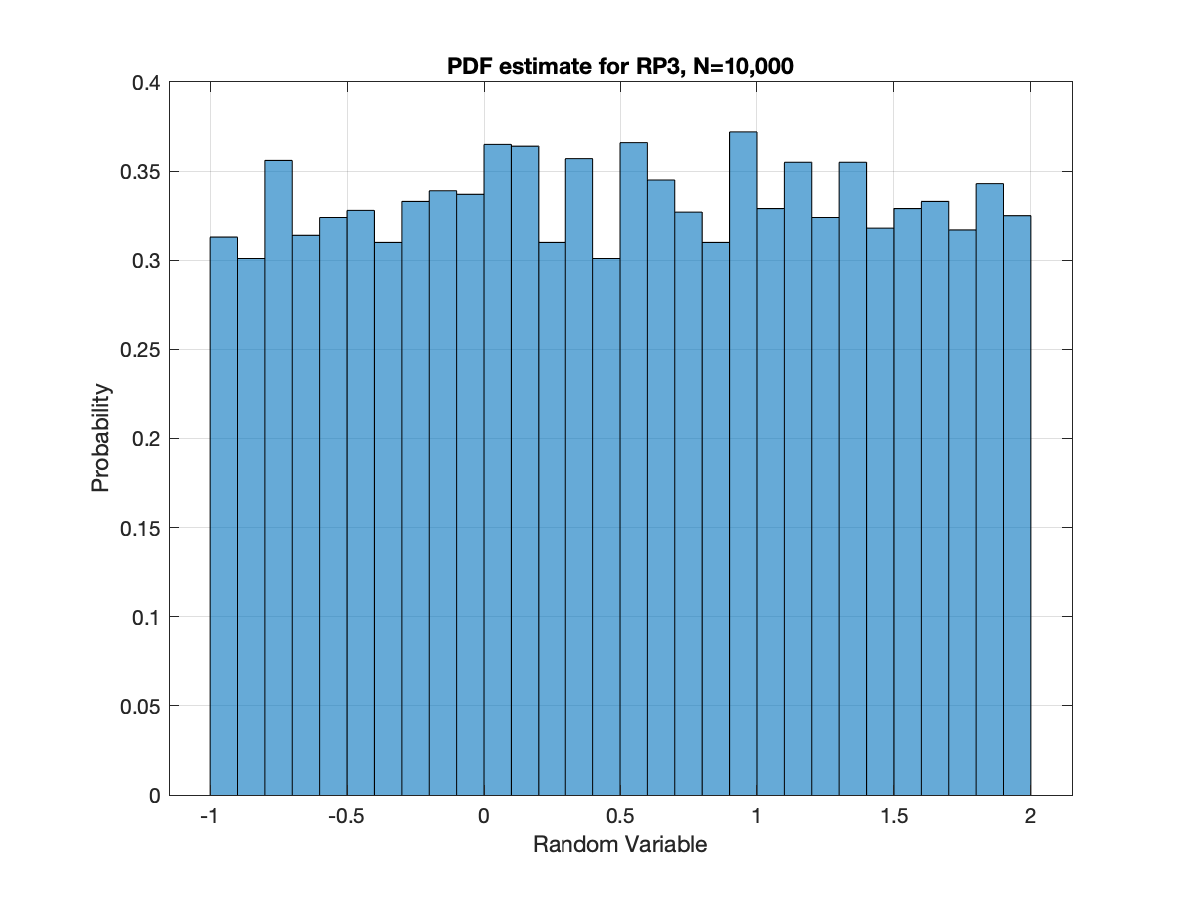
\includegraphics[width=\linewidth]{assignment1figs/rp310000}  
  \caption{10,000-sample realisation}
\end{subfigure}
\caption{Estimated PDFs of RP3}
\label{fig:rps}
\end{figure}
\noindent
It is clear that as the data length increases, the function better approximates the PDF of the process (which is a uniform distribution \textit{U}[-1,2] with constant value 0.333).

\subsubsection{Non-stationary processes}

As defined at the beginning of this section, a process is stationary if its PDF is constant in time. For this reason, the function written here could not accurately estimate the PDF of a non-stationary signal. A non-stationary process whose mean changes from 0 to 1 at N = 500 would essentially have two separate PDFS- one for $0\leq N < 500$ and one for $500 < N \leq 1000$. The only way to usefully apply the function written here would be to split the signal accordingly and apply the function to the two separate PDFs.
